\documentclass{article}

	\usepackage[margin=1in]{geometry}
	
	\usepackage[backend=bibtex, style=authoryear]{biblatex}
		
	\addbibresource{sources/sources.bib}
	\usepackage{hyperref}
	
			\title{\textsc{Neural Networks for Computed Tomography Imaging Spectrographs}}
			\date{\today}
			\author{Roy Smart \\ \url{roy.smart@montana.edu} \\ Montana State University, Department of Physics \\ Bozeman, MT 59717, USA}
			
	\usepackage{float}
	\usepackage{graphicx}
	\usepackage{subcaption}


\begin{document}

	\maketitle
	
	\tableofcontents
	
	\begin{abstract}
		
	\end{abstract}
		
	
	\section{Problem Statement}
		\subsection{Background}
		
			Spectrometers are important tools for solar astronomy. This is due to the fact that the Sun has a complex spectral structure, composing of numerous emission and absorption lines exhibiting variations in linewidth, mean wavelength and intensity.
			
			 Many spectrographic structures such as explosive events, first described by (\cite{dere1}), have yet to be fully explained, indicating that there is still much to be learned concerning the spectral structure of the sun.
			
			Conventional spectrographs such as \textit{IRIS}, split light into its component spectra using a diffraction grating and then use a slit to restrict the spatial field of view along the dispersion direction of the diffraction grating (\cite{De Pontieu2014}). This configuration yields images that represent the intensity of the light source as a 1D function of space (perpendicular to the dispersion direction) and a 1D function of wavelength. To acquire intensity information along the dispersion direction, conventional spectrographs are often operated in raster mode, where the slit is scanned parallel to the dispersion direction. This process builds up a \textit{spatial-spectral cube}, which contains the intensity of the light source as a 2D function of space and a 1D function of wavelength. Unfortunately the cube acquired through the process of rastering is not cotemporal, i.e. each of the images within the cube was taken at a different time, governed by the readout speed of the imager and the scanning speed of the slit. 		
		
			Computed tomography imaging spectrographs (CTISs) are a relatively new type of instrument that has been independently developed by multiple parties including: \cite{Okamoto:91}, \cite{bulygin:92}, \cite{Descour:95}, and \cite{kankel1}. This type of instrument promises to recover a cotemporal, spatial-spectral cube. CTISs accomplish this using a diffraction grating, similar to those used by conventional spectrographs, but unlike conventional spectrographs, CTISs are not equipped with a slit, allowing them to observe a wide field of view in both spatial directions. Without the slit, the spectral and spatial information from the light source is convolved into a single image. Since this convolution operation is not easily inverted, images are formed in multiple diffraction orders to provide enough information to reconstruct the spatial-spectral cube (\cite{inversion}).	
			 
		\subsection{Inversion}
		
			Computing the spatial spectral cube using images formed at multiple diffraction orders can be interpreted as a classic 3D tomography problem where $N$ projections are taken through a translucent 3D object in $x$, $y$ and $\lambda$ space (\cite{Bulygin:05}).
			\begin{figure}[h!]
				\centering
				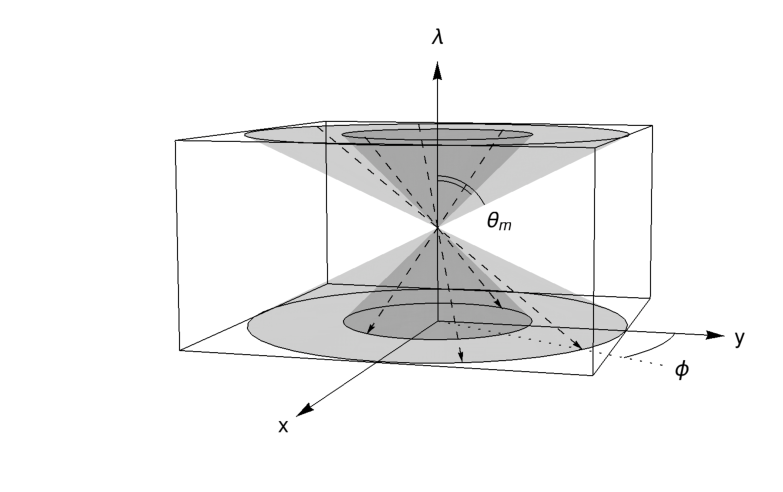
\includegraphics[width=0.75\textwidth]{figures/tomography}
				\caption{Geometry of the inversion problem for CTIS interpreted as a 3D tomography problem. $\theta_m$ describes the angle of the tomographic projection at each diffraction order and takes on discrete values, visualized by the nested cones. $\phi$ describes the dispersion direction and accepts continuous values. The four dotted lines are examples of particular projections through the spatial-spectal cube. Figure adapted from \cite{Bulygin:05}}
				\label{tomography}
			\end{figure}
			
			Using this representation, we can write the intensity in each order, $I_m$, of an object $v(x,y,\lambda)$ viewed by a CTIS in terms of the intergral equation provided by \cite{fox1}
			\begin{equation}
				I_m (x',y') = \int_B v(x' - \lambda \tan \theta_m \cos \phi, \; y' - \lambda \tan \theta_m \sin \phi, \; \lambda) \; d\lambda,
				\label{tomo_eqn}
			\end{equation}
			where $x'$ and $y'$ are image coordinates and $B$ is the passband of the instrument. Equation \ref{tomo_eqn} is a Fredholm integral equation of the first kind (\cite{RHB}) with a projection kernel. Our goal is then to invert Equation \ref{tomo_eqn} to recover the object $v(x,y,\lambda)$.
			
			The CTISs developed by Charles Kankelborg and his research group only take between $N=3$ and $N=6$ projections through the spatial-spectral cube. This limited number of projections does not provide enough information to completely reconstruct the spatial-spectral cube, i.e. in the case of the CTISs discussed below (MOSES and ESIS), inverting Equation \ref{tomo_eqn} is an ill-posed problem (\cite{inversion}). We can see this by noting that for a spatial spectral cube of length $L$ in both spatial directions, and a depth $M$ in the spectral direction the amount of information in the cube is $I_c = L^2 \times M$ and the the information provided by all the projections is $I_p = L^2 \times N$. Therefore, an inversion algorithm must to use physical constraints to have enough information to reconstruct the spatial-spectral cube (\cite{inversion}). In Section \ref{pwork} we will briefly explore advantages and disadvantages of the physical constraints used by current inversion algorithms, and in Section \ref{prop_sol} we will propose to use machine learning algorithms to approximate these physical constraints and solve the inversion problem.
			
		\subsection{Current and Planned CTISs}

			In the sections below, we will conduct a limited overview of the current and planned CTISs designed and built by Charles Kankelborg and his research group. A brief understanding of the optical system of each instrument will be helpful to understanding the goals of this proposal. 

			Each of the instuments in the succeeding sections is designed to fly on a Black Brant IX sounding rocket launched from White Sands Missile Range. Additionally, each instrument is constructed with a narrow passband in EUV. This narrow passband aims to alleviate intractability of the inversion process.

			\subsubsection{MOSES}

				The Multi-Order Solar EUV Spectrograph (MOSES) has successfully undertaken two flights. The first flight occurred in 2005 and observed the Sun in He \textsc{ii} 304 \AA (\cite{fox1}) while the second flight was just recently completed in 2015 and observed the Sun in He VII 465 \AA (\cite{smart1}). 
				
				MOSES is a CTIS that uses a single concave diffraction grating to produce images in three spectral orders, $m=-1,0,1$, as in Figure \ref{optics} (\cite{kankel1}). 		
				\begin{figure}[h!]
					\centering
					\begin{subfigure}[t]{0.49\textwidth}
						\centering
						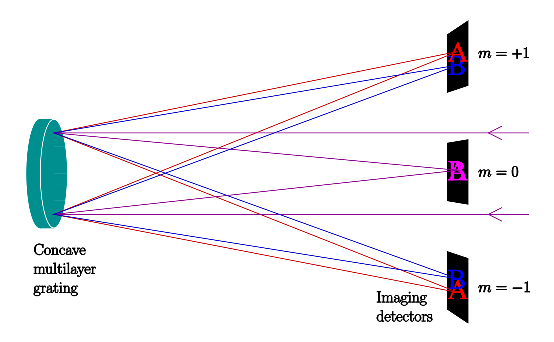
\includegraphics[height=2in]{figures/concave}
						\caption{Sketch of the optical system of MOSES}
						\label{optics}
					\end{subfigure}	
					~
					\begin{subfigure}[t]{0.49\textwidth}
						\centering
						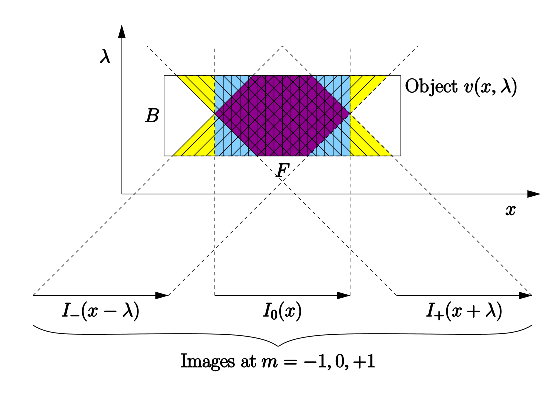
\includegraphics[height=2in]{figures/moses_cube}
						\caption{The analogue of Figure \ref{tomography} for the MOSES instrument.}
						\label{moses_tomo}
					\end{subfigure}	
					\caption{Two diagrams used to visualize the imaging system of the MOSES instrument. Figure \ref{optics} demonstrates how a bimodal spectral signal (a red `A' and a blue `B') are dispersed through the optical system. Figure \ref{moses_tomo} imagines the MOSES optical system as a 2D tomographic projection through a spatial-spectral cube. Figures courtesy of \cite{fox1}????}
				\end{figure}
				Since the diffraction grating of MOSES has rulings along only one direction, the dispersion is only in one direction. In the parlance of Figure \ref{tomography}, $\phi$ is restricted to the values of 0 and $\pi$ and then, without loss of generality, we can represent the 3D projections of Figure \ref{tomography} as 2D projections through a plane, as in Figure \ref{moses_tomo}.
				
				MOSES presents several challenges against achieving an accurate inversion. The most prevalent of these is the large, unknown point-spread function (PSF) of the instrument. The scale of this PSF is a compromise that allows MOSES to form images in three diffraction orders from a single optic (\cite{kankel1}).

			\subsubsection{ESIS}
			
				The EUV Snapshot Imaging Spectrograph (ESIS) is the next generation of a CTIS developed by Kankelborg and his research group. This instrument will be equipped with one large focusing primary mirror, and small, dedicated diffraction gratings for each detector. The first flight is planned for 2019 and the instrument will be equipped with four detectors to image the $m=1$ order in four separate dispersion directions. After the first flight has been completed, the system will undergo upgrades to install two additional gratings and detectors for a total of six tomographic projections. 
				\begin{figure}[h!]
					\centering
					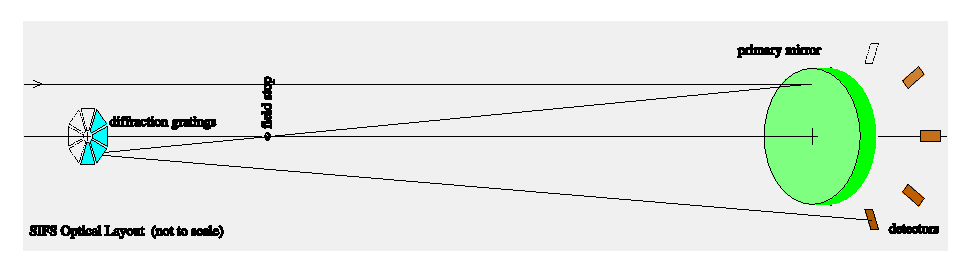
\includegraphics[width=0.8\textwidth]{figures/esis}
					\caption{A sketch following a single ray through the ESIS optical system. Image courtesy of Charles Kankelborg???}
					\label{esis_sketch}
				\end{figure}
				
				The tomographic projections of the ESIS instrument can be visualized in terms of Figure 1. The dedicated diffraction gratings are arranged in an octagonal pattern, producing projections at $\phi = 0, \; \pi/8, \; \pi/4, \; 3 \pi / 8, \; \pi /2, \; 5 \pi /8$ and $3 \pi /4$. Since these projections are not all in the same plane (unlike the MOSES arrangement), the inversion problem cannot be reduced to two dimensions and must be solved in 3D.
			
		\subsection{Previous Work}
			\label{pwork}
			
			The task of inverting MOSES data has already been undertaken by several research projects (\cite{inversion}, \cite{fox1}). These efforts have resulted in a \textit{de facto} standard inversion algorithm known as the Smooth Algebraic Reconstruction Technique (SMART). This inversion algorithm is based on an established technique for solving limited-angle computed tomography problems (\cite{Gordon70}) and has proved to be very successful in recovering line profiles and doppler shifts from MOSES data (SOURCE???).
			
			Unfortunately, it has proven difficult to convince SMART to produce physical inversions across the entire MOSES dataset. This unphysicality is mainly produced by an artifacts known colloquially as \textit{plaid}, visualized in Figure \ref{plaid}.
			\begin{figure}[h!]
				\centering
				\includegraphics[width=0.3\textwidth]{figures/plaid}
				\caption{An example of plaid produced by SMART. Image courtesy of Thomas Rust.}
				\label{plaid}
			\end{figure}
			Plaid is likely to be produced whenever a bright object in the spatial-spectral cube is imaged against a dark background. As an example, in Figure \ref{esis_sketch} we can see that the bright object in the center has been blurred at the angles: $\theta=-\pi/4, \; 0,$ and $\pi/4$ (with respect to the vertical). Such structures are obviously unphysical, and an inversion technique that is resistant to plaid would be useful to CTIS astronomy because...
		\subsection{Project Goals}
	\section{Proposed Solution}
		\label{prop_sol}
		\subsection{Introduction to Neural Networks}
		
			
		
		\subsection{Inversion Using Neural Networks}
		\subsection{Preliminary Results}
	\section{Relevance to Heliophysics}
	\section{Project Timeline}
	

	\printbibliography

	
\end{document}

